%!TEX root = ../DSGEnotes.tex
\chapter{将DSGE模型和实际数据联系起来}
\label{sec:connection}

第一部分讨论了在参数已经被赋值的前提下,如何近似求解DSGE模型。这一部分讨论如何基于实际观测到的数据,为DSGE模型的参数复制,并判断DSGE模型在何种程度上再现了经济现实。具体说来,大概有以下几个问题:
\begin{itemize}
  \item 如何基于观测到的(宏观)经济数据,估计DSGE模型中的参数值?
  \item 含有估计参数的DSGE模型(以下简称估计DSGE模型),可以在多大程度上反映观测数据的核心特征?
  \item 估计DSGE模型对于解释以下经济现象有何启发?如经济周期波动的成因、外甥冲击的影响、宏观经济政策变化的效果、时间序列数据的未来走势等。
  \item 在存在不确定性的情况下,如何更有效度量参数,和制定更恰当的DSGE模型的量化政策建议?
\end{itemize}

为了回答这些问题,我们首先建立一个典型的DSGE模型\todo{1},随后讨论该模型的性质\todo{2}。DSGE模型生成的模拟时间序列数据(以下简称模拟数据),包括全体的矩,协方差,光谱,冲击响应方程等,可以被视为是实际观测到的数据(以下简称观测数据)中特定样本同样具有的特征,二者的比较见\todo{3}。宏观经济学时间序列中含有的一些趋势中,有些能为DSGE模型所反映出来,有些则不能,相关讨论见\todo{4}。

在掌握宏观计量经济学基础知识(PHD最初几年学习)的基础上,关于DSGE模型估计的基础教科书可参考如\cite{Canova:2011vi}\todo{DeJong and Dave (2007)}。近年来DSGE估计方面的研究进展很快,下文将介绍一系列"标准方法",如
\begin{itemize}
  \item DSGE模型的识别
  \item 对识别稳健(identification-robust)的频率学派推断
  \item 贝叶斯分析中的马尔科夫链——蒙特卡洛方法(Marcov Chain Monte Carlo, MCMC)\citep{Herbst:2015wh}
  \item 此外还讨论了经济计量推断中误设定问题的后果,和频率学派的若干方法等。
\end{itemize}

\section{典型DSGE模型}
\label{sec:stylized-dsge-model}
整个第\ref{sec:estimation-dsge}部分基于一个对数线性化形式(可参考Remark \ref{remark:loglinearization})的新凯恩斯主义DSGE模型(New Keynesian-DSGE)展开讨论。这个模型来自\cite{DelNegro:2008de},做了一些参数简化\citep{Smets:2003ic, Christiano:2005ib},以下简称典型DSGE模型。

模型分为5个部门,分别是家庭部门,中间产品生产部门,最终产品生产部门,负责制定货币政策的中央银行,和负责制定财务政策的公共部门。4个外生冲击分别是技术进步冲击$z_{t}$,劳动——休闲偏好冲击$\phi_{t}$,加成定价格(price markup)冲击$\lambda_{t}$,货币政策冲击$\epsilon_{R,t}$。

最终产品生产率水平$Z_{t}$设为外生,是一个带漂移(drift)的随机游走(random walk)\index{random walk \dotfill 随机游走}过程
\begin{equation}
  \label{sec:stylized-productivity-level}
  \begin{split}
      & \log Z_{t} = \log Z_{t-1} + \log \gamma + z_{t}, \\
      & z_{t} = \rho_{z} z_{t-1} + \sigma_{z} \epsilon_{z,t},
  \end{split}
\end{equation}

生产率过程$Z_{t}$使得产出$X_{t}$和实际工资$X_{t}$呈现随机趋势过程(stochastic trend process)\index{sthochastic trend process \dotfill 随机趋势过程},因此需要去趋势(第\ref{sec:pta-non-lin-sys-steady-state}节),作如下定义:
\begin{equation}
  \label{eq:stylized-detrending-def}
  \begin{split}
    x_{t} \equiv \frac{X_{t}}{Z_{t}}, \quad w_{t} \equiv \frac{W_{t}}{Z_{t}}.
  \end{split}
\end{equation}

定义如下稳定状态(第\ref{sec:scaled-variables}节)
\begin{equation}
  \label{eq:stylized-ss-def}
  \begin{split}
    \bar{x}_{t} = x^{*}, \quad \bar{w} = \overline{lsh} = \frac{1}{1+\lambda}, \quad \overline{pi} = \pi^{*}, \quad \overline{R} = \pi^{*} \frac{\gamma}{\beta}
  \end{split},
\end{equation}
其中
\begin{itemize}
  \item 系数$\lambda$表示中间产品垄断生产者的稳态加成率,
  \item 系数$\beta$表示家庭的时间贴现,
  \item 系数$\gamma$是技术进步的稳态增长率,
  \item 稳定状态下,市场工资率等于全部收入中劳动者的分成$\overline{w}=\overline{lsh}$,
  \item 自由参数$\pi^{*}$可理解为中央银行设定的目标通胀率,
  \item 自由参数$x^{*}$原则上可以由家庭部门效用函数最大化决策中,对劳动的负效率和休闲的效用之间的权衡所计算得到,
  \item 均衡条件下产品的使用$\bar{x} = \bar{c}$。
\end{itemize}

\subsection{对数线性化均衡条件}
\label{sec:stylized-loglin-equilibra}

定义一组变量,用上角标表示其距离稳态值的对数偏离
\begin{equation}
  \label{eq:stylized-deviation}
  \begin{split}
    & \hat{x}_{t} = \log \left( \frac{x_{t}}{\overline{x}} \right), \\
    & \hat{w}_{t} = \log \left( \frac{w_{t}}{\overline{w}_{t}} \right), \\
    & \hat{\pi}_{t} = \log \left( \frac{\pi_{t}}{\overline{\pi}} \right), \\
    & \hat{R}_{t} = \log \left( \frac{R_{t}}{\overline{R}} \right),
  \end{split}
\end{equation}
由此可得典型DSGE模型的一系列均衡条件。

家庭部门跨期消费的欧拉等式
\begin{equation}
  \label{eq:stylized-hh-euler}
  \hat{x}_{t} = E_{t} \left[
  \hat{x}_{t+1}  + \hat{\pi}_{t} + z_{t+1} - \hat{R}_{t}
  \right],
\end{equation}
上式中出现对未来期技术进步冲击的期望$z_{t+1}$是因为欧拉等式反映产出(消费)距其稳态的对数线性化偏离,而产出的跨期变化受到随机技术趋势$Z_{t}$的影响。

假定不存在工资粘性(wage rigidities,第\ref{sec:hh-labor-contractors}节,更详细内容可参考\cite{Erceg:2000dm})。根据欧拉等式\eqref{eq:stylized-hh-euler}可得劳动力供应的决定式
\begin{equation}
  \label{eq:stylized-labor-supply}
  \hat{w}_{t} = \left( 1 + \nu \right) \hat{x}_{t} + \phi_{t},
\end{equation}
其中$\hat{x}_{t} \propto \widehat{L}_{t}$见\eqref{eq:stylized-intm-ss-produc}。$1/\left( 1 + \nu \right)$是劳动力供应的Frisch弹性系数(第\ref{sec:Frish-elasticity}节)。外生偏好冲击$\phi_{t}$
影响劳动力供应,满足如下AR(1)过程
\begin{equation}
  \label{eq:stylized-preference-shock-process}
  \phi_{t} = \rho_{\phi} \phi_{t-1} + \sigma_{\phi} \epsilon_{\phi,t}.
\end{equation}

中间产品生产者$j$,从家庭部门雇佣劳动力生产差异化中间产品$j$,对应线性生产技术
\begin{equation}
  \label{eq:stylized-intm-production-function}
  X_{t}(j) = Z_{t} L_{t}(j),
\end{equation}
作去趋势处理,并沿稳态值做对数线性化,得生产函数
\begin{equation}
  \label{eq:stylized-intm-ss-produc}
  \hat{x}_{t}(j) = \hat{L}_{t}(j).
\end{equation}

中间产品种类的差异化导致$j$的垄断竞争地位。垄断定价策略使得经济系统中存在名义价格粘性(nominal price rigidity),可用Calvo定价机制来反映\citep{Calvo:1983uq}。每一期$t$,$j$有$\xi_{p}$概率不能调整价格,$1 - \xi_{p}$概率可以调整价格。在可以调整价格的情况下,
$j$依据前向型定价策略,追求他在未来一段时间$t+s$之内的期望利润之和的最大化,直到$t+s+1$期他能再次调整价格为止。

最终产品生产者购买各种中间产品,将它们组合起来从事最终产品的生产,生产技术表现为CES形式,市场形式表现为完全竞争。

中间品部门和最终产品部门的最优决策组合起来,构成新凯恩斯主义菲利普斯曲线(New Keynesian Philips Curve, NKPC, 参考笔记第\pageref{eq:log-lin-reset-price-inflation-gap}页\index{New Keynesian Philips Curve (NKPC) \dotfill 新凯恩斯主义菲利普斯曲线})
\begin{equation}
  \label{eq:stylized-nkpc}
  \hat{\pi}_{t} = \beta E_{t} \hat{\pi}_{t+1}
  + \kappa_{p} \left( \hat{w}_{t} + \lambda_{t} \right), \quad \kappa_{p} \equiv \frac{1 - \zeta_{p}}{\zeta_{p}}\left( 1 - \zeta_{p} \beta \right),
\end{equation}
其中对价格加成的外部冲击$\lambda_{t}$设满足AR(1)过程
\begin{equation}
  \label{eq:stylized-shock-markup}
  \lambda_{t} = \rho_{\lambda} \lambda_{t-1} + \sigma_{\lambda} \epsilon_{\lambda,t}.
\end{equation}

经济体中总量约束条件的计算,具体来说,首先将总产出和产出的使用联系起来
\begin{equation}
  \label{eq:stylized-output-inandout}
  \hat{x}_{t} = \hat{c}_{t},
\end{equation}
齐次将劳动力的总需求和总产出联系起来。基于这样的总资源约束条件,可得
\begin{equation}
  \label{eq:stylized-agg-labor-w}
  \widehat{lsh}_{t} = \hat{w}_{t}.
\end{equation}

中央银行根据市场上反馈的信息,设定当期名义利率
\begin{equation}
  \label{eq:stylized-bank-rate}
  \hat{R}_{t} = \psi \hat{\pi}_{t} + \sigma_{R} \epsilon_{R,t}, \quad \psi = \frac{1}{\beta},
\end{equation}
这也是做了相当程度的简化。讨论货币政策的DSGE模型常常要引入利率的平滑机制,以及央行在制定货币政策是常常也需要考虑其他一些反映实际经济运行状况的指标如实际产出、潜在产出等(第\ref{sec:output-gap}节),又称泰勒法则(Taylor's rule),如见第\ref{seq:Taylor-Rule}节。外甥货币政策冲击$\epsilon_{R,t}$用于反映无法提前预知的系统性偏差。假定$\psi = \frac {1}{\beta}$时为了确保这样一组含有理性预期的线性方程系统,有且只有一个稳定解(理性期望模型的求解,见第\ref{sec:rational-exp-chap}章。)。

公共部门的主要工作是决定债务水平和一揽子税等,使得政府的预算约束条件得到满足。本模型中假定稳定状态下债务为$0$,总税收等于总转移支付,因而在均衡条件中可以不考虑。

\subsection{模型求解}
\label{sec:stylized-solution}
我们从整个经济系统中选取四个变量作为核心状态变量,进行系统缩减,以减轻计算负担(第\ref{sec:pj-approximation-tips-reduction}节)。由前述对数线性化的系统结构可见,四个运动法则方程$\left\{ \hat{x}_{t}, \widehat{lsh}_{t}, \hat{\pi}_{t}, \hat{R}_{t} \right\}$构成的缩减系统也是线性的。以下依次说明。

\subsubsection{产出的运动法则}
\label{sec:stylized-solution-x}

将泰勒法则\eqref{eq:stylized-bank-rate}代入欧拉等式
\eqref{eq:stylized-hh-euler}以消除名义利率$\hat{R}_{t}$
\begin{equation}
  \label{eq:stylized-euler-taylor-nor}
  \hat{x}_{t} = E_{t} \hat{x}_{t+1}
  - \underbrace{
  \left( \frac{1}{\beta} \hat{\pi}_{t} - E_{t} \hat{\pi}_{t+1} \right)
  }_{\eqqcolon \mathcal{A}}
  - \sigma_{R} \epsilon_{R,t}  + E_{t} z_{t+1},
\end{equation}
根据NKPC\eqref{eq:stylized-nkpc}和劳动力供应的决策式\eqref{eq:stylized-labor-supply}有
\begin{equation}
  \label{eq:stylized-nkpc-labor-supply}
  \mathcal{A} = \frac{1}{\beta} \hat{\pi}_{t} - E_{t} \hat{\pi}_{t+1}
  = \frac{\kappa_{p}}{\beta} \left( \hat{w}_{t} + \lambda_{t} \right)
  = \frac{\kappa_{p}}{\beta}
  \left[\left( 1 + \nu \right) \hat{x}_{t} + \phi_{t} + \lambda_{t}
  \right],
\end{equation}
\eqref{eq:stylized-euler-taylor-nor}因此变为
\begin{equation}
  \label{eq:stylized-euler-taylor-nor-reduce}
\begin{split}
  & \hat{x}_{t} = E_{t} \hat{x}_{t+1} -
  \left\{
  \frac{\kappa_{p}}{\beta}
  \left[
  \left( 1 + \nu \right) \hat{x}_{t} + \phi_{t} + \lambda_{t}
  \right]
  + \sigma_{R} \epsilon_{R,t}
  \right\}
  + E_{t} z_{t+1}, \\
  & \hookrightarrow
  \underbrace{
  \left[
  1 + \frac{\kappa_{p}}{\beta} \left( 1 + \nu \right)
  \right]
  }
  \hat{x}_{t} = E_{t} \hat{x}_{t+1} - \frac{\kappa_{p}}{\beta} \left( \phi_{t} + \lambda_{t} \right) - \sigma_{R} \epsilon_{R,t} + E_{t} z_{t+1}, \\
  & \hookrightarrow
  \hat{x}_{t} = \psi_{p} E_{t} \hat{x}_{t+1} - \frac{\kappa_{p} \psi_{p}}{\beta} \left( \phi_{t} + \lambda_{t} \right) - \psi_{p} \sigma_{R} \epsilon_{R,t} + \psi_{p} E_{t} z_{t+1}, \quad \psi_{p} \coloneqq \left[
  1 + \frac{\kappa_{p}}{\beta} \left( 1 + \nu \right)
  \right] \in [0,1],
\end{split}
\end{equation}
不难看出,产出的运动法则表示为一个含有期望的线性差分方程。由此我们将$\hat{x}_{t}$表示为线性决策形式(decision rule)
\begin{equation}
  \label{eq:stylized-output-decision-rule}
\begin{split}
  & \hat{x}_{t} \coloneqq \hat{x}_{t} \left( \phi_{t}, \lambda_{t}, z_{t}, \epsilon_{R,t} \right)
  = x_{\phi} \phi_{t} + x_{\lambda} \lambda_{t} + x_{z} z_{t} + x_{\epsilon_{R}} \epsilon_{R,t}, \\
  & x_{\phi} = - \frac{\psi_{p} \kappa_{p}}{\beta} \frac{1}{1 - \psi_{p} \rho_{\phi}}, \\
  & x_{\lambda} = - \frac{\psi_{p} \kappa_{p}}{\beta} \frac{1}{1 - \psi_{p} \rho_{\lambda}}, \\
  & x_{z} = \frac{
  \rho_{z} \psi_{p}
  }{
  1 - \psi_{p} \rho_{z}
  }, \\
  & x_{\epsilon_{R}} = - \psi_{p} \sigma_{R},
\end{split}
\end{equation}
作为泛函形式$E_{t} \mathcal{H} \left( \hat{x}_{t} \left( \phi_{t}, \lambda_{t}, z_{t}, \epsilon_{R,t} \right) \right) = 0$的解:
\begin{equation}
  \label{eq:stylized-output-functional-h}
\begin{split}
E_{t}
\left[
\hat{x} \left( \phi_{t}, \lambda_{t}, z_{t}, \epsilon_{R,t} \right)
- \psi_{p} \hat{x}
\begin{pmatrix}
  \rho_{\phi} \phi_{t} + \sigma_{\phi} \epsilon_{\phi, t+1}, \\
  \rho_{\lambda} \lambda_{t} + \sigma_{\lambda} \epsilon_{\lambda, t+1}, \\
  \rho_{z} z_{t} + \sigma_{z} \epsilon_{z,t+1}, \\
  \epsilon_{R,t+1}
\end{pmatrix}
+
\frac{\psi_{p} \kappa_{p}}{\beta} \left( \phi_{t} + \lambda_{t} \right)
+ \psi_{p} \sigma_{R} \epsilon_{R,t}
- \psi_{p} E_{t} z_{t+1}
\right] =0.
\end{split}
\end{equation}

\subsubsection{劳动收入份额的运动法则}
\label{sec:stylized-solution-lsh}
将劳动力供应的决定式\eqref{eq:stylized-labor-supply}和\eqref{eq:stylized-agg-labor-w}可得
\begin{equation*}
  \widehat{lsh}_{t} = \left[ \left( 1 + \nu \right) \hat{x}_{t} \right] + \phi_{t},
\end{equation*}
引入\eqref{eq:stylized-output-decision-rule},用$\hat{x}_{t} \left( \phi_{t}, \lambda_{t}, z_{t}, \epsilon_{R,t} \right)$替代掉$\hat{x}_{t}$,可得劳动收入份额的线性决策式
\begin{equation}
  \label{eq:stylized-labor-share-decision-rule}
\begin{split}
  \widehat{lsh}_{t}  & \coloneqq \widehat{lsh}_{t} \left( \phi_{t}, \lambda_{t}, z_{t}, \epsilon_{R,t} \right) \\
  & = \left[ \left( 1 + \nu \right) x_{\phi} + 1 \right] \phi_{t}
  + \left( 1 + \nu \right) x_{\lambda} \lambda_{t}
  + \left( 1 + \nu \right) x_{z} z_{t}
  + \left( 1 + \nu \right) x_{\epsilon_{R}} \epsilon_{R,t}.
\end{split}
\end{equation}

\subsubsection{通货膨胀率的运动法则}
\label{sec:stylized-solution-inflation}

\eqref{eq:stylized-labor-share-decision-rule}代回NKPC \eqref{eq:stylized-nkpc},用收入份额的线性决策式$\widehat{lsh}_{t} \left( \phi_{t}, \lambda_{t}, z_{t}, \epsilon_{R,t}  \right)$替代$\hat{w}_{t}$。
将通货膨胀率$\hat{\pi}_{t}$表示为近似线性形式$\hat{\pi}_{t} \left( \phi_{t}, \lambda_{t}, z_{t}, \epsilon_{R,t} \right)$,作为泛函
$E_{t} \mathcal{H} \hat{\pi}_{t} \left( \phi_{t}, \lambda_{t}, z_{t}, \epsilon_{R,t} \right) = 0$
的解
\begin{equation}
  \label{eq:stylized-inflation-functional-h}
\begin{split}
   E_{t} \left[
   \hat{\pi} \left( \phi_{t}, \lambda_{t}, z_{t}, \epsilon_{R,t} \right)
   - \beta \hat{\pi}
   \begin{pmatrix}
   \rho_{\phi} \phi_{t} + \sigma_{\phi} \epsilon_{\phi, t+1},\\
   \rho_{\lambda} \lambda + \sigma_{\lambda} \epsilon_{\lambda, t+1}, \\
   \rho_{z} z_{t} + \sigma_{z} \epsilon_{z,t+1}, \\
   \epsilon_{R, t+1}
   \end{pmatrix}
   - \kappa_{p}
   \underbrace{
   \widehat{lsh} \left( \phi_{t}, \lambda_{t}, z_{t}, \epsilon_{R,t} \right)
   }_{\eqref{eq:stylized-labor-share-decision-rule}}
   - \kappa_{p} \lambda_{t}
   \right],
\end{split}
\end{equation}
进而可得通货膨胀率的线性决策式
\begin{equation}
\label{eq:stylized-inflation-decision-rule}
\begin{split}
  \hat{\pi}_{t}  =  \hat{\pi} \left( \phi_{t}, \lambda_{t}, z_{t}, \epsilon_{R,t} \right) = & \frac{\kappa_{p}}{1 - \beta \rho_{\phi}} \left[ 1 + \left( 1 + \nu \right) x_{\phi} \right] \phi_{t}
  + \frac{\kappa_{p}}{1 - \beta \rho_{\lambda}} \left[ 1 + \left( 1 + \nu \right) x_{\lambda} \right] \lambda_{t} \\
  & + \frac{\kappa_{p}}{1 - \beta \rho_{z}} \left( 1 + \nu \right) x_{z} z_{t}
  + \kappa_{p} \left( 1 + \nu \right) x_{\epsilon_{R}} \epsilon_{R,t}
\end{split}
\end{equation}


\subsubsection{利率的运动法则}
\label{sec:stylized-solution-return-rate}
将\eqref{eq:stylized-inflation-decision-rule}代入泰勒法则\eqref{eq:stylized-bank-rate},用线性近似决策式$\hat{\pi}_{t} \left( \phi_{t}, \lambda_{t}, z_{t}, \epsilon_{R,t}  \right)$ 替代 $\hat{\pi}_{t}$,可得
\begin{equation}
   \label{eq:stylized-return-rate-decision-rule}
   \begin{split}
     \hat{R}_{t} =
     & \frac{\kappa_{p}}{\beta} \frac{1}{1 - \beta \rho_{\phi}}
     \left[ 1 + \left( 1 + \nu \right) x_{\phi} \right] \phi_{t}
     + \frac{\kappa_{p}}{\beta} \frac{1}{1 - \beta \rho_{\lambda}}
     \left[ 1 + \left( 1 + \nu \right) x_{\lambda} \right] \lambda_{t} \\
     & + \frac{\kappa_{p}}{\beta} \frac{1}{1 - \beta \rho_{z}}
     \left( 1 + \nu \right) x_{z} z_{t}
     + \left[ \frac{\kappa_{p}}{\beta}  \left( 1 + \nu \right) x_{\epsilon_{R}} + \sigma_{R} \right] \epsilon_{R,t}.
   \end{split}
\end{equation}

\subsubsection{外生冲击}
\label{sec:stylized-solution-shocks}
外生冲击$\left\{ \epsilon_{z_{t}}, \phi_{t}, \lambda_{t} \right\}$的运动法则分别由
\eqref{sec:stylized-productivity-level}
,\eqref{eq:stylized-preference-shock-process}
,\eqref{eq:stylized-shock-markup}给出,假定$\left\{ \epsilon_{R,t}, \epsilon_{z,t} \epsilon_{\phi, t}, \epsilon_{\lambda, t} \right\} $都是鞅差序列(Martingale Difference Sequence, MDS, Definition \ref{definition:martingale-difference-sequence})。

\begin{definition}[鞅差序列]
  \label{definition:martingale-difference-sequence}
  概率论中,假定一个定义在概率空间$\left( \omega, F, P \right)$中的随机序列$X = \left\{ x(n) \right\}_{n \ge 0}$,其中$F=\left\{ F(n) \right\}$是一个上升$\sigma$代数族(Definition \ref{definition:measure-sigma-algebra})。如果以下条件成立,那么我们称$X$为一个鞅差序列(Martingale Difference Sequence, MDS)\index{Martingale Difference Sequence (MDS) \dotfill 鞅差序列}:
  \begin{enumerate}
    \item $X$是$F$-适应的,即对任一$n \ge 0$,$X(n)$都是$F(n)$-可测度的,
    \item 对于任一$n \ge 0$,$X(n)$都可积,
    \item 对任一$n \ge 0$,满足$E \left[ X(n+1) | F(n) \right]=0, \, a.s.$,其中a.s.表示几乎总是(almost surely)。
  \end{enumerate}
\end{definition}

\subsection{状态——空间表现式}
\label{sec:stylized-ssrep}
为了更好的比较模拟数据与观测数据,需要对变量做处理。测量方程(measurement equation)\index{measurement equation \dotfill 测量方程}表现为以下形式
\begin{equation}
  \label{eq:stylized-ssrep-measurement-equations}
  \begin{split}
    \log \left( \frac{X_{t}}{X_{t-1}} \right) & = \hat{x}_{t} - \hat{x}_{t-1} + z_{t} + \log \gamma, \\
    \log \left( lsh_{t} \right) & = \widehat{lsh}_{t} + \log \left( lsh \right), \\
    \log \pi_{t} & = \hat{\pi}_{t} + \log \pi^{*}, \\
    \log R_{t} & = \hat{R}_{t} + \log \left( \frac{\pi^{*} \gamma }{\beta} \right).
  \end{split}
\end{equation}

通过测量方程的转换,我们可以将DSGE模型的模拟数据表示为状态空间模型的形式\cite[Ch. 6]{Shumway:2017ej}。具体说来,定义一组状态变量组成的向量$s_{t}$,和由13个参数构成的参数向量$\theta$
\begin{equation}
  \label{eq:stylized-ssrep-state-vector-def}
  \begin{split}
    \underbrace{
    s_{t}
    }_{\left[ n_{s} \times 1 \right]}
    & \equiv \left[
    \phi_{t}, \lambda_{t}, z_{t}, \epsilon_{R,t}, \hat{x}_{t-1}
    \right]^{\top}, \\
    \underbrace{
    \theta
    }_{\left[ 13 \times 1 \right]}
    & \equiv \left[
    \beta, \gamma, \lambda, \pi^{*}, \xi_{p}, \nu, \rho_{\phi}, \rho_{\lambda}, \rho_{z}, \sigma_{\phi}, \sigma_{\lambda}, \sigma_{z}, \sigma_{R}
    \right]^{\top}.
  \end{split}
\end{equation}

这样,可以将状态转移方程(state transition equation)表示如下
\begin{equation}
  \label{eq:stylized-ssrep-state-transition-equation}
  s_{t} = \phi_{1} \left( \theta \right) s_{t-1} + \phi_{\epsilon} \left( \theta \right) \epsilon_{t},
\end{equation}
其中
\begin{itemize}
  \item  预测误差向量$\epsilon_{t}$

  \begin{equation*}
    \underbrace{
    \epsilon_{t}
    }_{\left[ n_{\epsilon} \times 1 \right]}
    \equiv \left[ \epsilon_{\phi,t}, \epsilon_{\lambda,t}, \epsilon_{z,t}, \epsilon_{R,t} \right]^{\top},
  \end{equation*}
    \item $\phi_{1} \left( \theta \right)$和$\phi_{\epsilon} \left( \theta \right)$是系数矩阵,矩阵中的元素值反映以下几组关系
    \begin{itemize}
      \item $\phi_{t} \leftrightarrow \phi_{t-1}$, \eqref{eq:stylized-preference-shock-process}
      \item $\lambda_{t} \leftrightarrow \lambda_{t-1}$, \eqref{eq:stylized-shock-markup}
      \item $z_{t} \leftrightarrow z_{t-1}$,\eqref{sec:stylized-productivity-level}
      \item $\epsilon_{R,t} \equiv \epsilon_{R,t}$
      \item $\hat{x}_{t-1}$的决定式,\eqref{eq:stylized-euler-taylor-nor-reduce}。
    \end{itemize}
\end{itemize}

另一方面,对于观测数据,定义为向量$y_{t}$
\begin{equation}
  \label{eq:stylized-observed-vector-y}
  \underbrace{
  y_{t}
  }_{\left[ n_{y} \times 1 \right]}
   \equiv
   \underbrace{
   M_{y}^{\top}
   }_{\left[ n_{y} \times 4 \right]}
  \left[
  \log \left( \frac{X_{t}}{X_{t-1}} \right), \log \, lsh_{t}, \log \pi_{t}, \log R_{t}
  \right]^{\top},
\end{equation}
其中$M_{y}^{\top}$是一个选择矩阵(selection matrix),用于选择系数矩阵$\psi_{0} \left( \theta \right), \, \psi_{1} \left( \theta \right)$中的行。这样,将观测数据的测量方程表示为
\begin{equation}
  \label{eq:stylized-observed-measurement-equation}
  y_{t} = \psi_{0} \left( \theta \right) + \psi_{1} \left( \theta \right) s_{t},
\end{equation}
其中$s_{t}$由\eqref{eq:stylized-ssrep-state-transition-equation}定义,其值由四条运动法则组成的近似线性系统所给出,\eqref{eq:stylized-output-decision-rule},
\eqref{eq:stylized-labor-share-decision-rule},
\eqref{eq:stylized-inflation-decision-rule},
\eqref{eq:stylized-return-rate-decision-rule}
;系数矩阵$  \psi_{0} \left( \theta \right), \, \psi_{1} \left( \theta \right) $可由\eqref{eq:stylized-ssrep-measurement-equations}计算求得。

\subsubsection{从DSGE模型到状态空间模型}
\label{sec:stylized-dsge-to-ssrep}
这样,典型DSGE模型所对应的状态——空间模型为如下表达式:
\begin{equation*}
  \begin{split}
    y_{t} & = \psi_{0} \left( \theta \right) + \psi_{1} \left( \theta \right) s_{t}, \\
    s_{t} & = \phi_{1} \left( \theta \right) s_{t-1} + \phi_{\epsilon} \left( \theta \right) \epsilon_{t},
  \end{split}
\end{equation*}
其中系数矩阵分别为
\begin{equation*}
  \begin{split}
    \psi_{0} \left( \theta \right) & = M_{y}^{\top}
    \begin{pmatrix}
      \log \gamma \\
      \log \left( lsh \right) \\
      \log \pi^{*} \\
      \log \left( \frac{\gamma \pi^{*}}{\beta} \right)
    \end{pmatrix}, \\
    \psi_{1} \left( \theta \right) & = M_{y}^{\top}
    \begin{pmatrix}
      x_{\phi} & x_{\lambda} & x_{z} + 1 & x_{\epsilon_{R}} & -1 \\
      1 + \left( 1 + \nu \right) x_{\phi} &
      \left( 1 + \nu \right) x_{\lambda} &
      \left( 1 + \nu \right) x_{z}&
      \left( 1 + \nu \right) x_{\epsilon_{R}} &
      0 \\
      \frac{\kappa_{p}}{1 - \beta \rho_{\phi}} \left[ 1 + \left( 1 + \nu \right) x_{\phi} \right] &
      \frac{\kappa_{p}}{1 - \beta \rho_{\lambda}} \left[ 1 + \left( 1 + \nu \right) x_{\lambda} \right] &
      \frac{\kappa_{p}}{1 - \beta \rho_{z}} \left( 1 + \nu \right) x_{z}  &
      \kappa_{p} \left( 1 + \nu \right) x_{\epsilon_{R}} &
      0 \\
      \frac{\kappa_{p} }{\beta \left( 1 - \beta \rho_{\phi} \right)}
      \left[
      1 + \left( 1 + \nu \right) x_{\phi}
      \right] &
      \frac{\kappa_{p} }{\beta \left( 1 - \beta \rho_{\lambda} \right)}
      \left[
      1 + \left( 1 + \nu \right) x_{\lambda}
      \right] &
      \frac{\kappa_{p} }{\beta \left( 1 - \beta \rho_{z} \right)}
      \left( 1 + \nu \right) x_{z} &
      \frac{\kappa_{p}}{\beta} \left( 1 + \nu \right) x_{\epsilon_{R}} + \sigma_{R} &
      0
    \end{pmatrix}, \\
    \phi_{1} \left( \theta \right) & =
    \begin{pmatrix}
      \rho_{\phi} & 0 & 0 & 0 & 0 \\
      0 & \rho_{\lambda} & 0 & 0 & 0 \\
      0 & 0 & \rho_{z} & 0 & 0 \\
      0 & 0 & 0 & 0 & 0 \\
      x_{\phi} & x_{\lambda} & x_{z} & x_{\epsilon_{R}} & 0
    \end{pmatrix}, \\
    \phi_{\epsilon} \left( \theta \right) & =
    \begin{pmatrix}
      \sigma_{\phi} & 0 & 0 & 0 \\
      0 & \sigma_{\lambda} & 0 & 0 \\
      0 & 0 & \sigma_{z} & 0 \\
      0 & 0 & 0 & 1 \\
      0 & 0 & 0 & 0
    \end{pmatrix},
  \end{split}
\end{equation*}
其中$M_{y}^{\top}$是一个$\left[ n_{y} \times 4 \right]$的选择矩阵,用于选取$\psi_{0}\left( \theta \right)$和$\psi_{1}\left( \theta \right)$中的特定行。系数$\left\{ x_{\phi}, x_{\lambda}, x_{z}, x_{\epsilon_{R}} \right\}$的计算方法见\eqref{eq:stylized-output-decision-rule}。

由\eqref{eq:stylized-observed-measurement-equation} \eqref{eq:stylized-ssrep-state-transition-equation}所构成的典型DSGE模型的状态——空间表现形式,称为一系列后续计量经济分析的基础。它描述了在给定模型参数$\theta$的基础上,观测数据$y_{t}$和状态变量$s_{t}$的联合分布概率
\begin{equation}
  \label{eq:stylized-joint-probability-distribution}
  p \left( Y_{1:T}, S_{1:T}  | \theta \right)
  = \int
  \left[
  \prod_{t=1}^{T} p \left(y_{t} | s_{t}, \theta \right) p \left( s_{t} | s_{t-1}, \theta \right)
  \right] p  \left( S_{0} | \theta  \right) d S_{0} ,
\end{equation}
其中$Y_{1:T} = \left\{ y_{1}, \ldots, y_{t} \right\}, \, S_{1:T} = \left\{ s_{1}, \ldots, s_{t} \right\}$。状态变量集合$S_{1:T}$中,常常有一部分信息无法直接观测到,直接利用\eqref{eq:stylized-joint-probability-distribution}计算联合分布概率的思路很可能不可行。对此,常见的处理方法是,基于实际观测数据,计算边际分布概率$p \left( Y_{1:T} | \theta \right)$
\begin{equation}
  \label{eq:stylized-marginal-probability-distribution}
  p \left( Y_{1:T} | \theta \right) = \int p \left( Y_{1:T}, S_{t:T} | \theta \right) d S_{1:T}.
\end{equation}

边际分布概率$p \left( Y_{1:T} | \theta \right)$是一个关于$\theta$的方程,有时也称似然方程(likelihood function, 见第\ref{sec:mle}节),它在计量推断过程中的作用非常重要\todo{笔记打出来之后,是在sec 10,做一个ref}。

\begin{remark}[``状态"变量]
  来看以下两组变量,第一组是$\left\{ \phi_{t}, \lambda_{t}, z_{t}, \epsilon_{R,t} \right\}$,第二组是$s_{t} = \left\{ \phi_{t}, \lambda_{t}, z_{t}, \epsilon_{R,t}, \hat{x}_{t-1} \right\}$。前者是经济学意义上的状态变量,与经济系统中行为人的跨期最优决策有关。后者是计量经济学意义上的状态变量,用于将DSGE模型的近似解投进状态——空间表现式\eqref{eq:stylized-observed-measurement-equation} \eqref{eq:stylized-ssrep-state-transition-equation}中去。

  \begin{enumerate}
    \item 前者在我们的简单DSGE模型设定中,都假定是外生的。但一个更复杂的DSGE模型中,$s_{t}$完全可以包括其他一些内生变量如实物资本存量等。
    \item 测量方程\eqref{eq:stylized-observed-measurement-equation} \eqref{eq:stylized-ssrep-state-transition-equation}中产出的增速$\hat{x}_{t-1}$也可以用产出水平$x_{t-1}, \, x_{t-2}$来表示,如果用产出水平代替增速,就需要在参数向量中加入稳态产出$x^{*}$,在$s_{t}$中减去$\hat{x}_{t-1}$,加入$\log Z_{t}/\gamma^{t}$,以及在测量方程中产出的一项上,考虑到确定性趋势$\left( \log \gamma \right) t$的作用。
    \item 也可以在测量方程\eqref{eq:stylized-ssrep-state-transition-equation}中加入额外的测量误差项。
    \item 如果在前一阶段,对DSGE模型是作高阶扰动或者投影法的近似求解的,那么在这一阶段,随着状态变量$s_{t}$的定义越是精确,就越可能出现状态转移方程\eqref{eq:stylized-observed-measurement-equation}和测量方程\eqref{eq:stylized-ssrep-state-transition-equation}是非线性的情况。
  \end{enumerate}
\end{remark}

\section{模型的含义}
\label{sec:stylized-model-implications}
一旦我们对状态转移方程\eqref{eq:stylized-observed-measurement-equation}含有新息(innovation)的误差向量$\epsilon_{t}$的分布信息明确了(这反映在系数矩阵$\phi_{\epsilon} \left( \theta \right)$中),就可以最终确定DSGE模型中诸多变量的概率分步。由此,如果进一步将$\epsilon_{t}$的设为满足独立同分布
\begin{equation*}
  \epsilon_{t} \sim i.i.d. \, \mathcal{N} \left(0, I \right),
\end{equation*}
其中$I$是个单位矩阵,那么,基于这样的概率结构,我们很容易得DSGE模型的一组特征如下,这组特征有助于我们更好估计参数向量$\theta$的具体数值,以及模型的拟合度。本节介绍这些特征。

在介绍之前,出于简化模型的考虑,我们先对$\theta$系数值作校准,暂时赋予定值\todo{下文给出估计方法},见表 \ref{tab:stylized-parameter-calibration}。

\begin{table}[htbp]
\begin{center}
    \centering
    \caption{典型DSGE模型的参数校准}
    \label{tab:stylized-parameter-calibration}
    \begin{tabular}{lr|lr}
        \hline
        参数 & 值 & 参数 & 值 \\
        \hline
        $\beta$ & $1/1.01 $ & $\gamma$ & $\exp \left( 0.005 \right)$ \\
        $\lambda$ & 0.15	&  $\pi^{*}$ & $\exp \left( 0.005 \right)$ \\
        $\xi_{p} $ &	$0.65$ & $\nu $ & $0$ \\
        $\rho_{\phi}$ & $0.94$ &	$\rho_{\lambda}$ &	$0.88$ \\
        $\rho_{z}$ & $0.13$ & & \\
        $\sigma_{\phi}$ &	$0.01$	& $\sigma_{\lambda}$ &	$0.01$\\
        $\sigma_{z}$	& $0.01$	& $\sigma_{R}$ &	$0.01$ \\
        \hline
    \end{tabular}
\end{center}
\end{table}

\subsection{自协方差,预测误差方差}
\label{sec:stylized-ssrep-var}
DSGE模型能在多大程度上解释实际观测数据中的周期性波动?这就需要做模型精确度的分析,值得关注的特征是自协方差、预测误差方差。如前文所述,DSGE模型关注的主要对象时经济系统中的周期性波动。因此,模型中的方差(variances)、自相关(auto correlations)、互相关(cross correlations)等信息应当予以重点关注。

\subsubsection{协方差}
\label{sec:stylized-ssrep-covariance-lyapunov}
对于近似线性的DSGE模型,对应状态——空间表现形式\eqref{eq:stylized-observed-measurement-equation} \eqref{eq:stylized-ssrep-state-transition-equation},其自协方差方程(autocovariance)、跨协方差方程(crosscovariance)可表示为
\begin{equation}
  \label{eq:stylized-ssrep-autocov}
\begin{split}
    & \Gamma_{yy}\left( h \right) = E \left[ y_{t} y_{t-h} \right], \\
    & \Gamma_{ss} \left( h \right) = E \left[ s_{t} s_{t-h} \right], \\
    & \Gamma_{ys} \left( h \right) = E \left[ y_{t} s_{t-h}^{\top} \right],
\end{split}
\end{equation}
此外也假定预测误差满足
\begin{equation}
  \label{eq:stylized-ssrep-forecast-error-identity}
  E \left[ \epsilon_{t} \epsilon_{t}^{\top} \right] = I.
\end{equation}

那么,可以将$s_{t}$的协方差矩阵表示为如下李雅普诺夫方程(Lyapunov function)\index{Lyapunov function \dotfill 李雅普诺夫方程}的解\footnote{
将表\ref{tab:stylized-parameter-calibration}的校准参数值赋给状态——空间表现式
\eqref{eq:stylized-observed-measurement-equation}中的系数矩阵$\phi_{1}\left(\theta \right)$后,可得特征根(善用Mathematica!)
$Eigen = \left\{ 0.94,\, 0.88,\, 0.13,\, 0,\, 0 \right\}$,即$\left| Eigen \right| <1$。这表示$s_{t}$的$VAR(1)$运动式是协方差平稳的。}

\begin{equation}
  \label{eq:stylized-ssrep-lyapunov-func}
  \Gamma_{ss} \left( 0 \right) = \phi_{1} \Gamma_{ss} \left( 0 \right) \phi_{1}^{\top} + \phi_{\epsilon} \phi_{\epsilon}^{\top}
\end{equation}

\begin{algorithm}
  在Mathematica中,先计算$\phi_{\epsilon} \phi_{\epsilon}^{\top}$的值,随后用
\begin{mmaCell}{Input}
DiscreteLyapunovSolve[a,c]
\end{mmaCell}
来求解。Matlab中对应的命令是dylap。生成的$\Gamma_{ss} \left(0 \right)$为
\begin{equation*}
  \Gamma_{ss} \left(0 \right) =
  \begin{pmatrix}%{ccccc}
   -0.000859107 & 0. & 0. & 0. & 0.000619325 \\
   0. & -0.000443262 & 0. & 0. & 0.000242601 \\
   0. & 0. & -0.000101719 & 0. & \text{1.6265930319175398E-6} \\
   0. & 0. & 0. & -1. & 0. \\
   0.000619325 & 0.000242601 & \text{1.62659303191754E-6} & 0. &
     -0.000748026 \\
  \end{pmatrix}
\end{equation*}
\end{algorithm}

基于$\Gamma_{ss} \left(0 \right)$,可进一步计算$\Gamma_{ss}\left( h \right), \, h >0$
\begin{equation}
  \label{eq:stylized-ssrep-cov-ss-h}
  \Gamma_{ss}\left( h \right) = \phi_{1}^{h} \Gamma_{ss}\left( 0 \right).
\end{equation}

进一步,由测量方程\eqref{eq:stylized-observed-measurement-equation}可得$\Gamma_{yy} \left( h \right), \, \Gamma_{ys} \left( h \right)$的值
\begin{align}
  \label{eq:stylized-ssrep-cov-yy-h}
  \Gamma_{yy} \left( h \right) & = \psi_{1} \Gamma_{ss} \left( h \right) \psi_{1}^{\top}, \\
  \label{eq:stylized-ssrep-cov-ys-h}
   \Gamma_{ys} \left( h \right) & = \psi_{1} \Gamma_{ss} \left( h \right) \psi_{1}^{\top}.
\end{align}

有了这一系列协方差矩阵后,便可进一步计算相关和自相关矩阵。

\subsubsection{预测误差}
\label{sec:stylized-ssrep-covariance-forecast}
另一种求解思路是,将状态向量$s_{t}$理解为一组从$0$到无穷阶移动平均(moving average, MA)过程的和
\begin{equation}
  \label{eq:stylized-ssrep-ma}
\begin{split}
  y_{t} & = \psi_{0} + \psi_{1} s_{t} \\
  & = \psi_{0} + \psi_{1} \sum_{s=0}^{\infty} \phi_{1}^{s} \psi_{\epsilon} \epsilon_{t-s},
\end{split}
\end{equation}

在此基础上,可以计算如过去$t-h$期对当前$t$期的预测误差,定义为$e_{t | t-h}$
\begin{equation}
  \label{eq:stylized-ssrep-h-stepahead-forecast-error}
  e_{t | t-h} = y_{t} - E_{t-h} \left( y_{t} \right)
  = \psi_{1} \sum_{s=0}^{h-1} \psi_{1}^{s} \phi_{\epsilon} \epsilon_{t-s},
\end{equation}
又称h步前向预测误差(h-stepahead forecast error)。

那么可建立h步前向预测误差的协方差矩阵
\begin{equation}
  \label{eq:stylized-ssrep-h-stepahead-forecast-error-covariance}
  E \left[ e_{t | t-h} \, e_{t | t-h}^{\top} \right]
  = \psi_{1}
  \left(
  \sum_{s=0}^{h-1} \phi_{1}^{s} \phi_{\epsilon} \phi_{\epsilon}^{\top} \phi_{1}^{s, \top}
  \right) \psi_{1}^{T}.
\end{equation}

对\eqref{eq:stylized-ssrep-h-stepahead-forecast-error-covariance}取$h \rightarrow \infty$的极限,有
\begin{equation}
  \label{eq:stylized-ssrep-h-stepahead-forecast-error-covariance-infty}
  \lim_{h \rightarrow \infty} E \left[ e_{t | t-h} e_{t | t-h}^{\top} \right]
  \approx \Gamma_{ss} \left( 0 \right).
\end{equation}

那么在假定\eqref{eq:stylized-ssrep-forecast-error-identity}成立的前提下,可以进一步计算预测误差的协方差矩阵(协方阵)的分解如下。设$I^{(j)}$表示单位矩阵$I$的对角元素中,除了第$j$个元素之外的元素值都为$0$。那么$I$是全部$I^{(j)}$之和
\begin{equation}
  \label{eq:stylized-ssrep-forecast-cov-identity}
  I = \sum_{j=1}^{n_{\epsilon}} I^{(j)}, \quad j=1,\ldots,n_{\epsilon},
\end{equation}
那么编号为$j$的外生冲击,对观测数据的预测误差的影响表现为$e^{(j)}_{t|t-h}$
\begin{equation}
  \label{eq:stylized-ssrep-forecast-error-j}
  e^{(j)}_{t|t-h} = \psi_{1} \sum_{s=0}^{h-1} \phi_{1}^{s} \phi_{\epsilon} I^{(j)} \epsilon_{t-s}.
\end{equation}

第$j$个外生冲击的h步前向预测误差的协方差矩阵因此为
\begin{equation}
  \label{eq:stylized-ssrep-forecast-error-j-matrix}
  E \left[ e_{t | t-h}^{(j)} \, e_{t | t-h}^{(j), \top} \right]
  = \psi_{1}
  \left(
  \sum_{s=0}^{h-1} \phi_{1}^{s} \phi_{\epsilon} I^{(j)} \phi_{\epsilon}^{\top} \phi_{1}^{s, \top}
  \right) \psi_{1}^{T}.
\end{equation}

那么,$h$期第$j$个外生冲击,对$t$期第$i$个观测数据$y_{i,t}$的预测误差的影响(方差),表示为如下比值关系,定义为预测误差方差分解(forecast error variance decomposition, FEVD)
\begin{equation}
  \label{eq:stylized-ssrep-forecast-fevd}
  FEVD\left ( i,j,h \right) =
  \frac{
  \left[
  e^{(j)}_{t | t-h}
  \right]_{ii}
  }{
  \left[
  E \left[ e_{t|t-h} \, e_{t|t-h}^{\top} \right]
  \right]_{ii}
  }=
  \frac{
  \left[
  \psi_{1}
  \left(
  \sum_{s=0}^{h-1} \phi_{1}^{s} \phi_{\epsilon} I^{(j)} \phi_{\epsilon}^{\top} \phi_{1}^{s,\top}
  \right)
  \psi_{1}^{\top}
  \right]_{ii}
  }{
  \left[
  \psi_{1}
  \left(
  \sum_{s=0}^{h-1}
  \phi_{1}^{s} \phi_{\epsilon} \phi_{\epsilon}^{\top} \phi_{1}^{s,\top}
  \right)
  \psi_{1}^{\top}
  \right]_{ii}
  },
\end{equation}
其中$\left[ \cdot \right]_{ij}$表示矩阵的第$(i,j)$元素。

\begin{figure}[htbp]
  \caption{预测误差的方差分解}
  \centering
  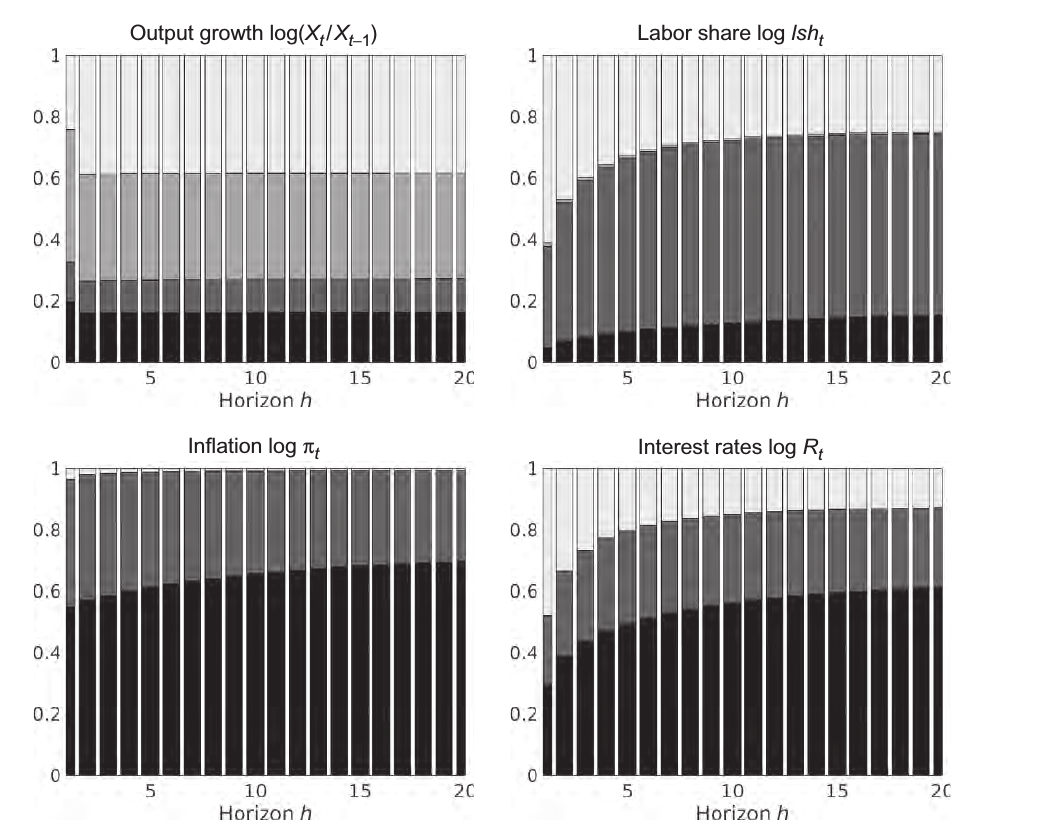
\includegraphics[width=12cm]{./Figures/20180401-fevd}
  \label{fig:stylized-ssrep-fevd}
%
%  \small{Source: PBOC.}
\end{figure}

图\ref{fig:stylized-ssrep-fevd}给出了4个冲击$\left\{ \phi_{t}, \lambda_{t}, z_{t}, \epsilon_{R,t} \right\}$对观测变量$\left\{ \log \left( X_{t}/X_{t-1} \right), \log lsh_{t}, \log \pi_{t}, \log R_{t} \right\}$的预测误差及其分解。每一单条(值为标准化的$1$)表示一个累积预测误差的方差分解,单条内分为四种颜色,从下倒上由深到浅依次表示偏好冲击$\phi_{t}$,价格加成冲击$\lambda_{t}$,技术冲击$z_{t}$,和货币政策冲击$\epsilon_{R,t}$。基于表\ref{tab:stylized-parameter-calibration}给出的校准参数值,不难看出
\begin{itemize}
  \item 产出增速的波动绝大多数归因于技术冲击$z_{t}$和货币政策冲击$\epsilon_{R,t}$,
  \item 劳动收入的波动主要归因于价格加成的冲击$\lambda_{t}$,并且从长期来看影响更为显著,
  \item 通货膨胀率和利率的波动收到偏好冲击$\phi_{t}$和价格加成冲击$\lambda_{t}$的强烈影响。
\end{itemize}


\subsection{光谱分析}
\label{sec:stylized-ssrep-spectral}

第\ref{sec:stylized-ssrep-var}节主要是从精确度的层面入手,分析预测误差的成因及影响。此外我们也可以从频率分析的角度入手\footnote{参考第\ref{sec:fourier-analysis}节。在时间序列分析中,频率域技术的应用有着悠久的历史,经典参考文献如\citep{Koopmans:1995vn, Diebold:2010ei}。}。先来看一个简单的线性周期模型,设$\left\{ y \right\}_{t}$是个矢量时间序列周期过程,满足
\begin{equation}
  \label{eq:stylized-ssrep-y}
\begin{split}
  y_{t} & = 2 \sum_{j=1}^{m} a_{j} \cos \left( \omega_{j} t + \theta_{j} \right) \\
  & = 2 \sum_{j=1}^{m} a_{j}
  \left[
  \cos \theta_{j} \, \cos \left( \omega_{j} t \right)
  - \sin \theta_{j} \sin \left( \omega_{j} t \right)
  \right], \quad \theta_{j} \sim i.i.d. \, U[-\pi, \pi], \, 0 \le \omega_{j} \le \omega_{j+1} \le \pi.
\end{split}
\end{equation}

随机变量$\theta_{j}$的导致$y_{t}$发生相位移动(phase shift)。为了简化表述,假定初始相位移动发生在无限久远之前。这样,\eqref{eq:stylized-ssrep-y}将实值域中的$y_{t}$理解为傅里叶域中一系列弦波曲线之和,这些波以不同的频率彼此区分。

$\omega_{j}$的单位往往与$t$的单位有关,后者在DSGE模型中设定,如以季度为时间单位,含有32个季度的数据,那么$\omega_{j} = \frac{2 \pi}{32}$。
一个常见的经济周期模型,可能会包含8到23个季度数据,对应的$\omega_{j} \in \left[ 0.196, 0.785 \right]$。

对于$\omega \in [ - \pi, \pi )$,时间序列$y_{t}$在傅里叶域中的光谱分布,可以表示为
\begin{equation}
  \label{sec:stylized-ssrep-fourier-y}
  \mathcal{F}_{yy} \left( \omega \right) = \sum_{j=-m}^{m}
  \mathbb{E} \left[ A \left( \omega_{j} \right) \,
  \overline{
  A \left( \omega_{j} \right)
  }
  \right]
  \mathbb{I} \left\{ \omega_{j} \le \omega \right\},
\end{equation}
\begin{itemize}
  \item $\overline{A \left( \omega_{j} \right)}$表示$A \left( \omega_{j} \right)$的复共轭(complex conjugate, 第\ref{sec:euler-complex-angle-conjugate}节)\index{complex conjugate \dotfill 复共轭}。
  \item $ \mathbb{I}(\cdot)$是一个指示方程(indicator function)\index{indicator function \dotfill 指示方程},满足
  \begin{equation}
    \label{eq:euler-complex-indicator-function-def}
    \mathbb{I} \left\{ \omega_{j} \le \omega \right\}
    = \begin{cases}
    1 & \text{如果}\left\{\omega_{j} \le \omega \right\} == TRUE, \\
    0 & \text{否则}
    \end{cases}.
  \end{equation}
\end{itemize}

如果$F_{yy} \left( \omega \right)$对$\omega$可导,那么其一阶导数就是光谱密度(spectral density)\index{spectral density \dotfill 光谱密度}方程$f_{yy} \left( \omega \right)$
\begin{equation}
  \label{eq:ssrep-spectral-density-function}
  f_{yy} \left( \omega \right) = \frac{\mathrm{d}}{\mathrm{d} \omega} F_{yy} \left( \omega \right).
\end{equation}

某个过程的光谱密度方程若是$f_{yy} \left( \omega \right)$ \eqref{eq:ssrep-spectral-density-function},那么该过程的协方差可以表示为$\Gamma_{yy} \left( h \right)$
\begin{equation}
  \label{eq:ssrep-spectral-covariance}
  \Gamma_{yy} \left( h \right) = \int_{(- \pi, \pi ]}
  \exp \left( i h \omega \right)
  f_{yy} \left( \omega \right) \, \mathrm{d} \omega.
\end{equation}

那么,线性周期方程$y_{t}$ \eqref{eq:stylized-ssrep-y}的自协方差$\Gamma_{yy} \left( h \right)$为
\begin{equation}
  \label{eq:stylized-ssrep-y-autocovariance}
  \Gamma_{yy} \left( h \right)
  = \sum_{j=-m}^{m} \mathbb{E} \left[ A \left( \omega_{j} \right) \, \overline{A \left( \omega_{j} \right)} \right] \exp \left( i h \omega \right).
\end{equation}

在给定光谱密度$f_{yy} \left( \omega \right)$的情况下,我们可以算得自协方差$\Gamma_{yy} \left( h \right)$。反之亦然,已知$\Gamma_{yy} \left( h \right)$,可求得光谱密度$f_{yy} \left( \omega \right)$
\begin{equation}
  \label{eq:stylized-ssrep-autocovariance-density}
  f_{yy} \left( \omega \right) = \frac{\mathrm{d}}{\mathrm{d} \omega} F_{yy} \left( \omega \right) = \frac{1}{2 \pi} \sum_{h=-\infty}^{\infty} \Gamma_{yy} \left( h \right) \exp \left( - i \omega h \right).
\end{equation}

结合自协方差数列$\Gamma_{yy} \left( h \right)$ \eqref{eq:ssrep-spectral-covariance}和光谱密度$f_{yy} \left( \omega \right)$ \eqref{eq:stylized-ssrep-autocovariance-density}不难看出,二者含有完全相同的信息(帕塞瓦尔定理, Theorem \ref{theorem:fourier-parseval-theorem})。

那么,回到典型DSGE模型的状态——空间表现式\eqref{eq:stylized-observed-measurement-equation} \eqref{eq:stylized-ssrep-state-transition-equation}
中,状态向量$s_{t}$的自协方差$\Gamma_{ss} \left( h \right)$由\eqref{eq:stylized-ssrep-cov-ss-h}计算而得,$\Gamma_{ss}\left( 0 \right)$由\eqref{eq:stylized-ssrep-lyapunov-func}计算而得。将它代入\eqref{eq:stylized-ssrep-autocovariance-density}可得状态向量$s_{t}$的光谱密度方程$f_{ss} \left( \omega \right)$
\begin{equation}
  \label{eq:stylized-ssrep-autocovariance-density-ss}
  \begin{split}
    f_{ss} \left( \omega \right)
    & = \frac{1}{2\pi} \sum_{h=-\infty}^{\infty} \Gamma_{ss} \left( h \right) \exp \left( - i \omega h \right) \\
    & = \frac{1}{2 \pi} \sum_{h=-\infty}^{\infty} \phi_{1}^{h} \Gamma_{ss} \left( 0 \right) \exp \left( - i \omega h \right) \\
    & = \frac{1}{2 \pi}
    \left[
    I - \phi_{1}^{\top} \exp \left( i \omega \right)
    \right]^{-1}
    \phi_{\epsilon} \phi_{\epsilon}^{\top}
    \left[
    I - \phi_{1} \exp \left( - i \omega \right)
    \right]^{-1}.
  \end{split}
\end{equation}

进而,第$j$个冲击对光谱密度$f_{ss} \left( \omega \right)$ \eqref{eq:stylized-ssrep-autocovariance-density-ss}的影响,记为$f_{ss}^{(j)} \left( \omega \right)$,计算如下
\begin{equation}
  \label{eq:stylized-ssrep-autocovariance-density-ss-j}
  f_{ss}^{(j)} \left( \omega \right) = \frac{1}{2 \pi}
  \left[
  I - \phi_{1}^{\top} \exp \left( i \omega \right)
  \right]^{-1}
  \phi_{\epsilon} I^{(j)} \phi_{\epsilon}^{\top}
  \left[
  I - \phi_{1} \exp \left( - i \omega \right)
  \right]^{-1},
\end{equation}
其中$I^{(j)}$的定义见\eqref{eq:stylized-ssrep-forecast-cov-identity}。

观测数据向量$y_{t}$的光谱密度方程$f_{yy} \left( \omega \right)$
\begin{equation}
  \label{eq:stylized-ssrep-autocovariance-density-yy}
  \begin{split}
    f_{yy} \left( \omega \right)
    = \psi_{1} f_{ss} \left( \omega \right) \psi_{1}^{\top},
  \end{split}
\end{equation}
第$j$个冲击对光谱密度$f_{yy} \left( \omega \right)$ \eqref{eq:stylized-ssrep-autocovariance-density-yy}的影响,记为$f_{yy}^{(j)} \left( \omega \right)$,计算如下
\begin{equation}
  \label{eq:stylized-ssrep-autocovariance-density-yy-j}
  f_{yy}^{(j)} \left( \omega \right)
  = \psi_{1} f_{ss}^{j} \left( \omega \right) \psi_{1}^{\top}.
\end{equation}
需要注意的是,光谱密度方程$f_{yy} \left( \omega \right)$是一个方阵,对角线元素$f_{yy}^{(j)}$反映第$j$个冲击的影响,典型DSGE模型中观测数据向量中含有4个变量的时间序列,分别是产出增速、劳动力收入份额、通货膨胀和利率,进而基于表\ref{tab:stylized-parameter-calibration}提供的参数校准,图  \ref{fig:stylized-ssrep-spectral-decomposition}
绘出4种冲击对4个观测变量的光谱密度分解,颜色由深到浅分别表示$\phi_{t}, \lambda_{t}, z_{t}, \epsilon_{R,t}$,4种冲击加总构成累积光谱密度,表现为图中的每条竖块。由于4个冲击彼此不相关,且均设为符合AR(1)过程,那么不难看出,在初始频率处光谱密度值最高(冲击的影响最大),随着频率的增大而逐渐衰减。

\begin{figure}[htbp]
  \caption{预测误差的方差分解}
  \centering
  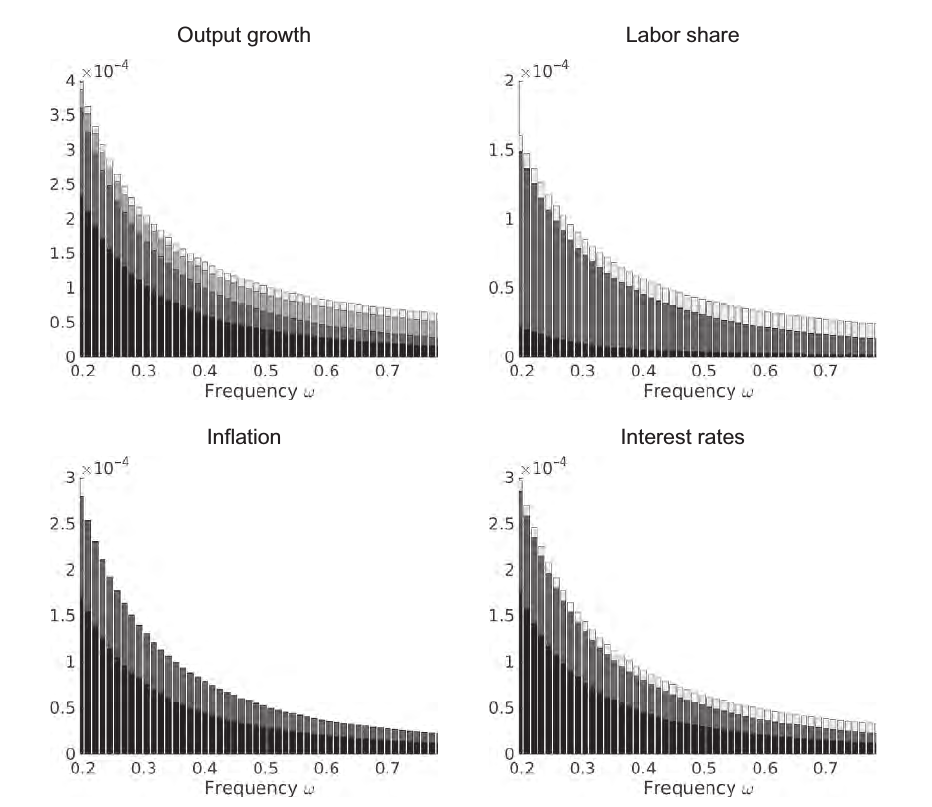
\includegraphics[width=12cm]{./Figures/20180403-spectral-decomposition}
  \label{fig:stylized-ssrep-spectral-decomposition}
%
%  \small{Source: PBOC.}
\end{figure}

\subsection{冲击响应方程}
\label{sec:stylized-ssrep-irfs}
研究外生冲击对经济系统的影响,一个重要的工具是冲击响应方程(impulse-response functions, IRFs)\index{impulse-response functions (IRFs) \dotfill 冲击响应方程}。DSGE模型中的冲击响应方程可以定义为以下两个条件期望之差
\begin{equation}
  \label{eq:stylized-ssrep-irfs-def}
  IRF \left( i, j, h | s_{t-1} \right) =
  E \left[ y_{i,t+h} | s_{t-1}, \epsilon_{j,t}=1 \right]
  - E \left[ y_{i,t+h} | s_{t-1} \right],
\end{equation}
两个条件期望
\begin{itemize}
  \item 相同之处:
  \begin{itemize}
    \item 都与上一期状态$s_{t-1}$有关,从而可以向前追溯到初始状态,
    \item 都与冲击$\epsilon_{t}$对随后$t+1,\ldots,t+h$期的持续影响(积分)有关,
  \end{itemize}
  \item 不同之处
  \begin{itemize}
    \item 前者还包括条件$\epsilon_{j,t}=1$,即$t$期第$j$个冲击出现,
    \item 后者则假定$\epsilon_{j,t}=0$,即即$t$期第$j$个冲击不发生。
  \end{itemize}
\end{itemize}

对于状态——空间形式表现的典型DSGE模型系统\eqref{eq:stylized-observed-measurement-equation} \eqref{eq:stylized-ssrep-state-transition-equation},由它的线性性质和分布性质$E \left[ \epsilon_{t+h} | s_{t-1} \right] = 0, \, h=0,1,\ldots $可得,第$j$个冲击的响应方程根据\eqref{eq:stylized-ssrep-irfs-def}写为
\begin{equation}
  \label{eq:stylized-ssrep-irfs}
  IRF \left( \cdot , j, h \right) =
  \frac{\partial}{\partial \epsilon_{j,t}} \psi_{1}
  = \psi_{1} \phi_{1}^{h} \left[ \phi_{\epsilon} \right]_{.j},
\end{equation}
上式中比起定义式\eqref{eq:stylized-ssrep-irfs-def}来省略掉了条件$| s_{t-1}$,是由于分布性质的假设。$\left[ \cdot \right]_{.j}$表示矩阵的第$j$列。

图\ref{fig:stylized-ssrep-irfs-output},以模型中内生变量产出增速$ 100 \times \log X_{t+h}/X_{t}$为例,依次绘出$t$期4种外生冲击的新息(innovation) $\epsilon_{\phi,t}, \, \epsilon_{\lambda,t}, \, \epsilon_{z,t}, \, \epsilon_{R,t}$在随后的$t+h, h=0,1,\ldots,20$期的影响。其中产出增速的线性近似决策式由\eqref{eq:stylized-output-decision-rule}给出,外生冲击的4个AR(1)过程由前节依次给定。不难看出
\begin{enumerate}
  \item 偏好冲击和价格加成的新息冲击产生负影响,产出随着时间变化逐渐恢复到稳态水平。
  \item 技术冲击的新息产生正影响,并且正影响是持续性的。
  \item 货币冲击新息的影响只持续1期。
\end{enumerate}

\begin{figure}[htbp]
  \caption{产出的冲击响应方程}
  \centering
  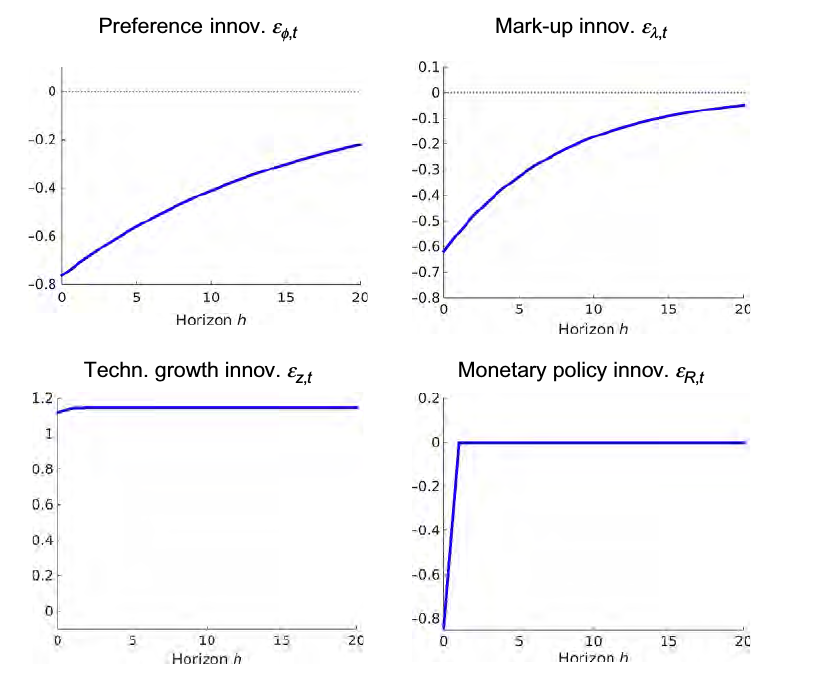
\includegraphics[width=12cm]{./Figures/20180403-irfs-output}
  \label{fig:stylized-ssrep-irfs-output}
%
%  \small{Source: PBOC.}
\end{figure}

\subsubsection{条件矩的限制}
\label{sec:stylized-ssrep-restrictions}
DSGE模型中的跨期最优决策,都是以条件矩限制(conditional moment restrictions)的形式出现的。例如NKPC式\eqref{eq:stylized-nkpc}意味着以下条件矩限制需要得到满足
\begin{equation}
  \label{eq:stylized-sspre-moment-nkpc}
  E_{t-1} \left[
  \hat{\pi}_{t-1} - \beta \hat{\pi}_{t} - \kappa_{p}
  \left(
  \widehat{lsh}_{t-1} + \lambda_{t-1}
  \right)
  \right] = 0.
\end{equation}

有条件的矩限制,可以用如下方法转换为一组无条件的矩限制所构成的向量。将全部过去时段的信息$\left\{ y_{\tau}, s_{\tau}, \epsilon_{\tau} \right\}_{\tau = - \infty}^{t}$定义为一个sigma代数族$\mathcal{F}_{t}$,进而定义一个$\mathcal{F}_{t}$—可测度的随机变量的向量$\widetilde{\mathcal{Z}}_{t}$(即是说$\widetilde{\mathcal{Z}}_{t}$的值可基于全部已有新息$\left\{ y_{\tau}, s_{\tau}, \epsilon_{\tau} \right\}_{\tau = - \infty}^{t}$而确定)。那么对于每一个已经确定了的$\widetilde{\mathcal{Z}}_{t-1}$,都有以下等式成立
\begin{equation}
  \label{eq:stylized-sspre-moment-nkpc-info-set}
\begin{split}
  & E \left[
  \widetilde{\mathcal{Z}}_{t-1}
  \left(
  \hat{\pi}_{t-1} - \beta \hat{\pi}_{t} - \kappa_{p}
  \left(
  \widehat{lsh}_{t-1} + \lambda_{t-1}
  \right)
  \right)
  \right] \\
  & = E \left[
  \widetilde{\mathcal{Z}}_{t-1}
  E_{t-1}
  \left[
  \left(
  \hat{\pi}_{t-1} - \beta \hat{\pi}_{t} - \kappa_{p}
  \left(
  \widehat{lsh}_{t-1} + \lambda_{t-1}
  \right)
  \right)
  \right]
  \right] = 0,
\end{split}
\end{equation}
其中$E_{t-1} \left[ \cdot \right] \equiv E \left[ \cdot | \mathcal{F}_{t-1} \right]$。需要指出的是,NKPC的矩条件中包括一个隐含变量(latent variable)\index{latent variable \dotfill 隐含变量}即当期价格加成冲击$\lambda_{t-1}$,是作决策时并不掌握的信息。这使得若直接利用\eqref{eq:stylized-sspre-moment-nkpc-info-set}来估计目标方程,可能会存在问题。

作为替代方案,可以考虑跨期消费的欧拉等式\eqref{eq:stylized-hh-euler},将$t$切换成$t-1$
\begin{equation*}
  E_{t-1} \left[
  \hat{x}_{t} - \hat{x}_{t-1}
  \right]
  + E_{t-1} \left[ z_{t} \right]
  + \hat{\pi}_{t-1} - \hat{R}_{t-1}=0,
\end{equation*}
由\eqref{eq:stylized-ssrep-measurement-equations}得到一组替换条件
\begin{equation*}
  \begin{split}
    E_{t-1} \left[
    \hat{x}_{t} - \hat{x}_{t-1}
    \right]
    + E_{t-1} \left[ z_{t} \right] & = E_{t-1} \log \left( \frac{X_{t}}{X_{t-1}} \right) - \log \gamma, \\
    \hat{\pi}_{t-1} & = \log \pi_{t-1} - \log \pi^{*}, \\
    \hat{R}_{t-1} & = \log R_{t-1} - \log \left( \frac{\pi^{*} \gamma }{\beta} \right),
  \end{split}
\end{equation*}
代回上式,得到消费欧拉等式的条件矩
\begin{equation}
  \label{eq:stylized-sspre-moment-euler-info-set}
  E_{t-1} \left[
  \log \left( \frac{X_{t}}{X_{t-1}} \right)
  + \log \pi_{t-1} - \log R_{t-1} - \log \left( \frac{1}{\beta} \right)
  \right]=0,
\end{equation}
稳态通货膨胀率$\pi^{*}$和稳态技术进步率$\gamma$被消掉;$\beta$参数的值在研究中被赋予;条件矩限制中只剩下了观测数据,而不再有隐含变量。

类似地,由\eqref{eq:stylized-bank-rate},将$t$切换为$t-1$,有
\begin{equation*}
  E_{t-1} \left[ \hat{R}_{t} - \psi \cdot \hat{\pi}_{t} - \sigma_{R} \epsilon_{R,t} \right]=0,
\end{equation*}

根据$\epsilon_{R,t}$是个鞅差序列MDS的假定(Definition \ref{definition:martingale-difference-sequence}),我们有
\begin{equation*}
  E_{t-1} \left[ \epsilon_{R,t} \right] = E \left[ \epsilon_{R,t} \right] = 0,
\end{equation*}
利用\eqref{eq:stylized-ssrep-measurement-equations}替换$\hat{R}_{t}$和$\hat{\pi}_{t}$,那么上式进一步调整为泰勒法则的条件矩
\begin{equation}
  \label{eq:stylized-sspre-moment-taylor-info-set}
  E_{t-1}
  \left[
  \log R_{t} - \frac{1}{\beta} \log \pi_{t} + \left( \frac{1 - \beta}{\beta} \right) \log \pi^{*} - \log \left( \frac{\gamma}{\beta} \right)
  \right] = 0,
\end{equation}
式中同样消除了隐含变量。

在此基础上,对于消费欧拉等式的条件矩\eqref{eq:stylized-sspre-moment-euler-info-set}和泰勒法则的条件矩\eqref{eq:stylized-sspre-moment-taylor-info-set},都可遵循\eqref{eq:stylized-sspre-moment-nkpc-info-set}的思路,利用一个$\mathcal{F}_{t-1}$——可测的随机向量$\widetilde{\mathcal{Z}}_{t-1}$,转换为无条件矩限制。

对于第\ref{sec:stylized-dsge-model}节的典型DSGE模型,具有定义良好的特点,从而在转换成状态——空间系统之后,可以直接用解析法求出自协方差矩阵、光谱密度、冲击响应方程等。利用这些信息,在对参数向量$\theta$赋值后,可进一步做数值计算。

对于一些特殊线性结构的DSGE模型,如果采用某些特定类型的扰动法去求近似解,也存在一些对应的解析方法去求解析矩条件,但适用范围有限\citep{Andreasen:2016cd}。对于更一般的非线性DSGE模型,我们往往要用蒙特卡洛法(Monte Carlo method)\index{Monte Carlo method \dotfill 蒙特卡洛法}作数值模拟来求系统的矩条件。例如,对一个DSGE模型的状态——空间表现式,首先基于解析模型设定中的分布信息,绘制初始状态向量$s_{0}$和新息矩阵$\epsilon_{t}$,然后通过仿真生成一组模拟数据$Y_{1:T}^{*}=\left\{ \right\}$,满足
\begin{equation}
  \label{eq:stylized-ssrep-simulation-mcmc}
  \frac{1}{T} \sum_{t=1}^{T} y_{t}^{*} \xrightarrow{s.s} E \left[ y_{t} \right],
\end{equation}
其中$a.s.$表示几乎总是(almost surely)\footnote{我们说一个随机变量数列$X_{T}$“几乎总是”收敛到一个有界的随机变量$X$,如果$X_{T}$不收敛至$X$的轨迹的概率为$0$。}。

蒙特卡洛模拟法的适用性前提之一是,根据DSGE模型的设定,(模拟)时间序列数据应当是严格平稳和严格遍历的。蒙特卡洛法的突出不足表现在,近似可能会有误差\todo{笔记敲到键盘里之后,做一个reference:如何通过对矩条件的仿真近似来估计参数向量$\theta$}。%sec11.2
